\documentclass[conference]{article} % IEEEtran
\IEEEoverridecommandlockouts
% The preceding line is only needed to identify funding in the first footnote. If that is unneeded, please comment it out.
\usepackage{cite}
\usepackage{amsmath,amssymb,amsfonts}
\DeclareMathOperator*{\argmax}{argmax}
\DeclareMathOperator*{\argmin}{argmin}
\DeclareMathOperator{\Tr}{Tr}
\DeclareMathOperator{\diag}{diag}
\usepackage{algorithmic}
\usepackage{graphicx}
\usepackage{textcomp}
\usepackage{xcolor}
\usepackage{tikz}
\def\BibTeX{{\rm B\kern-.05em{\sc i\kern-.025em b}\kern-.08em
    T\kern-.1667em\lower.7ex\hbox{E}\kern-.125emX}}
\begin{document}

\title{
% Graph Based Decomposition of a Single Robotic System Control with a Decentralized Network Control
% \\
% Perspectives on a Single Articulated Robotic System as a Graph Based Network System 

Graph-Based Dynamics and Network Control of a Single Articulated Robotic System

% Dynamics and Control of a Single Articulated Robot using Graph-Based Network Methods

% \\
% A New Perspective of a Single Articulated Robotic System as a Graph Based Network System
% {\footnotesize \textsuperscript{*}Note:}
\thanks{Identify applicable funding agency here. If none, delete this.}
}

\author{\IEEEauthorblockN{1\textsuperscript{st} Given Name Surname}
\IEEEauthorblockA{\textit{dept. name of organization (of Aff.)} \\
\textit{name of organization (of Aff.)}\\
City, Country \\
email address or ORCID}
\and
\IEEEauthorblockN{2\textsuperscript{nd} Given Name Surname}
\IEEEauthorblockA{\textit{dept. name of organization (of Aff.)} \\
\textit{name of organization (of Aff.)}\\
City, Country \\
email address or ORCID}
}

\maketitle

\begin{abstract}
Short summary of the paper
\end{abstract}

\section{Introduction}
Vector-network method, what is the same and different from that paper?
Why overparameterization?

\section{Preliminaries}
Talk about prereqs (Graph theory, definitions)

\section{Network Dynamics}
In order to explore this way of looking at robotic systems, we present a very simple class of systems in 2D space: a collection of $n$ point masses fixed together with $k$ massless rods, which act as distance constraints. Masses with multiple rods connected to them act as revolute joints. We define the Euler-Lagrange equation for this system as:
\begin{equation} \label{eq:EL}
    M\ddot{Q}+MG+\Gamma(Q,\dot{Q})=F
\end{equation}
where:
$$Q=\begin{bmatrix}
    x_1 & y_1\\
    \vdots & \vdots\\
    x_n & y_n
\end{bmatrix}=\begin{bmatrix}
    r_1^T\\ \vdots\\ r_n^T
\end{bmatrix}\in\mathbb{R}^{n\times2},\:
G=\begin{bmatrix}
    0 & g\\
    \vdots & \vdots\\
    0 & g
\end{bmatrix}\in\mathbb{R}^{n\times2}$$
$$M=\begin{bmatrix}
    m_1\\
    & \ddots\\
    & & m_n
\end{bmatrix}\in\mathbb{R}^{n\times n}$$
$$F=\begin{bmatrix}
    f_{1,x} & f_{1,y}\\
    \vdots & \vdots\\
    f_{n,x} & f_{n,y}
\end{bmatrix}\in\mathbb{R}^{n\times2}$$
and $\Gamma(Q,\dot{Q})\in\mathbb{R}^{n\times2}$ is the matrix of constraint forces. The goal of this section is to show how this matrix relates to and can be represented with a graph structure. We start by defining a network of constraints where the $n$ point masses represent nodes and the $k$ distance constraints represent edges. The incidence matrix of this graph can be written as:
$$D(G)= \begin{bmatrix}
    | & & |\\
    d_1 & \hdots & d_k\\
    | & & |
\end{bmatrix}\in\mathbb{R}^{n\times k}$$
where the column $d_i$ corresponds to the $i$th edge and contains a $1$ and $-1$ at the indices where masses are connected.

Continuing in the vein of graph theory, we can define an edge coordinates matrix given by the transformation:
$$Q_e=D(\mathcal{G})^TQ=\begin{bmatrix}
    r_{1e}^T\\ \vdots\\ r_{ke}^T
\end{bmatrix}\in\mathbb{R}^{k\times2}$$
$$r_{ie}=Q^Td_i$$
where each row $r_{ie}^T$ of $Q_e$ is the vector displacement between masses with a distance constraint. Therefore $\|r_{ie}\|=\ell_i$ is the constant length of the $i$th massless rod. We will refer to the rows of $Q$ as the node coordinates and the rows of $Q_e$ as the edge coordinates.

The constraint equations are written as:
$$h_i(Q)=\|Q^Td_i\|^2-\ell_i^2=0$$
$$\frac{dh_i}{dQ}=2Q^Td_id_i^T$$
Putting the constraints together, we define the constraint matrix as:
$$A(Q)\triangleq\frac{1}{2}\frac{dh}{dQ}=\begin{bmatrix}
    Q^Td_1d_1^T\\ \vdots\\ Q^Td_kd_k^T
\end{bmatrix}\in\mathbb{R}^{2k\times n}$$
We also define the vector of constraint forces $\lambda$ which are the magnitudes of the forces on the $k$ constraint rods:
$$\lambda=\begin{bmatrix}
    \lambda_1\\ \vdots\\ \lambda_k
\end{bmatrix}\in\mathbb{R}^{k\times 1}$$
Now we can begin to solve for $\Gamma$:
\begin{align*}
    \Gamma&=A(Q)^T(\lambda\otimes I_{2\times2})\\
    &=\begin{bmatrix}
        Q^Td_1d_1^T\\ \vdots\\ Q^Td_kd_k^T
    \end{bmatrix}^T\begin{bmatrix}
        \lambda_1I_{2\times2}\\ \vdots\\ \lambda_kI_{2\times2}
    \end{bmatrix}\\
    &=\begin{bmatrix}
        d_1d_1^TQ & \hdots & d_kd_k^TQ
    \end{bmatrix}\begin{bmatrix}
        \lambda_1I_{2\times2}\\ \vdots\\ \lambda_kI_{2\times2}
    \end{bmatrix}\\
    &= \sum_{i=1}^k d_i\lambda_id_i^TQ\\
    &= D(\mathcal{G})\Lambda D(\mathcal{G})^TQ\\
    &= L_w(\mathcal{G})Q
\end{align*}
*Talk about why this is interesting*
$$M\ddot{Q}+MG+D(\mathcal{G})\Lambda D(\mathcal{G})^TQ=F$$

Now, we must solve for $\lambda$.
$$\ddot{Q}=-G+M^{-1}(F-D(\mathcal{G})\Lambda D(\mathcal{G})^TQ)$$
$$\begin{bmatrix}
    d_1^T\dot{Q}Q^Td_1\\
    \vdots\\
    d_k^T\dot{Q}Q^Td_k\\
\end{bmatrix}=0$$
Take the derivative:
$$\begin{bmatrix}
    d_1^T\ddot{Q}Q^Td_1+\|\dot{Q}^Td_1\|^2\\
    \vdots\\
    d_k^T\ddot{Q}Q^Td_k+\|\dot{Q}^Td_k\|^2\\
\end{bmatrix}=0$$
$$\begin{bmatrix}
    d_1^TM^{-1}(F-D(\mathcal{G})\Lambda D(\mathcal{G})^TQ)Q^Td_1+\|\dot{r}_{1e}\|^2\\
    \vdots\\
    d_k^TM^{-1}(F-D(\mathcal{G})\Lambda D(\mathcal{G})^TQ)Q^Td_k+\|\dot{r}_{ke}\|^2\\
\end{bmatrix}=0$$
Note that $d_i^TG=0$
$$\begin{bmatrix}
    d_1^TM^{-1}D(\mathcal{G})\Lambda Q_er_{1e}\\
    \vdots\\
    d_k^TM^{-1}D(\mathcal{G})\Lambda Q_er_{ke}\\
\end{bmatrix}=\begin{bmatrix}
    d_1^TM^{-1}Fr_{1e}+\|\dot{r}_{1e}\|^2\\
    \vdots\\
    d_k^TM^{-1}Fr_{ke}+\|\dot{r}_{ke}\|^2\\
\end{bmatrix}$$
$$\begin{bmatrix}
    \Tr\left(Q_er_{1e}d_1^TM^{-1}D(\mathcal{G})\Lambda\right)\\
    \vdots\\
    \Tr\left(Q_er_{ke}d_k^TM^{-1}D(\mathcal{G})\Lambda\right)\\
\end{bmatrix}=\begin{bmatrix}
    d_1^TM^{-1}Fr_{1e}+\|\dot{r}_{1e}\|^2\\
    \vdots\\
    d_k^TM^{-1}Fr_{ke}+\|\dot{r}_{ke}\|^2\\
\end{bmatrix}$$
Notice the $i$th row of the left side of the equation is the trace of the outer product of the vectors $Q_er_{ie}$ and $D(\mathcal{G})^TM^{-1}d_i$ times the diagonal matrix $\Lambda$. This is equivalent to the Hadamard (elementwise) product of $Q_er_{ie}$ and $D(\mathcal{G})^TM^{-1}d_i$, inner product with $\lambda$.
$$\begin{bmatrix}
    \left(D(\mathcal{G})^TM^{-1}d_1\odot Q_er_{1e}\right)^T\\
    \vdots\\
    \left(D(\mathcal{G})^TM^{-1}d_k\odot Q_er_{ke}\right)^T\\
\end{bmatrix}\lambda=\begin{bmatrix}
    d_1^TM^{-1}Fr_{1e}+\|\dot{r}_{1e}\|^2\\
    \vdots\\
    d_k^TM^{-1}Fr_{ke}+\|\dot{r}_{ke}\|^2\\
\end{bmatrix}$$
$$\left(D(\mathcal{G})^TM^{-1}D(\mathcal{G})\odot Q_eQ_e^T\right)\lambda=\diag\left(D(\mathcal{G})^TM^{-1}FQ_e^T+\dot{Q}_e\dot{Q}_e^T\right)$$
If the constraints are independent, a solution for $\lambda$ exists.
\begin{equation} \label{eq:lambda}
    \lambda=\left(D(\mathcal{G})^TM^{-1}D(\mathcal{G})\odot Q_eQ_e^T\right)^{-1}\diag\left(D(\mathcal{G})^TM^{-1}FQ_e^T+\dot{Q}_e\dot{Q}_e^T\right)
\end{equation}
Note the equation for $\lambda$ depends only on edge coordinates and their derivatives.

\section{Network Control}
Sometimes it may be useful to directly control the edge coordinates and their velocities without regard for the node coordinates. For example, we may want to control the orientation of the rods that connect masses together and their angular velocities while paying no attention to where the robot exists in space or what forces may be acting on the entire robot (such as gravity). We propose a modification to the Euler-Lagrange equation given by equation \ref{eq:EL} by multiplying it by the edge transformation matrix $D(\mathcal{G})^T$:
$$\ddot{Q}_e+D(\mathcal{G})^TM^{-1}\Gamma(Q_e,\dot{Q}_e)=D(\mathcal{G})^TM^{-1}F$$
Now, since the equation only contains edge coordinates, their velocities, and force inputs, we can employ a variety of methods to control the edge coordinates to a desired trajectory. We will use the feedback linearization technique in this paper for simplicity. We propose the controller:
\begin{multline} \label{eq:controller}
    D(\mathcal{G})^TM^{-1}F=-k_1(Q_e-Q_{e,d})-k_2(\dot{Q}_e-\dot{Q}_{e,d})+\ddot{Q}_{e,d}\\
    +D(\mathcal{G})^TM^{-1}\Gamma(Q_e, \dot{Q}_e)
\end{multline}
In general, $D(\mathcal{G})$ is not full rank, therefore we cannot write an equation for $F$. We will look at how to solve for the control input $F$ through examples.

\section{Results}
\subsection{Two link pendulum}
\begin{figure}[htbp]
    \centering
    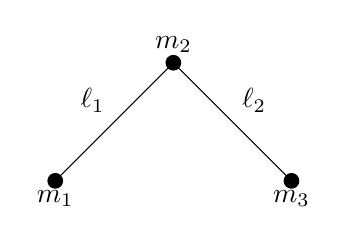
\begin{tikzpicture}
        \fill[black] (-1.5, -1.5) circle (1mm) node[anchor=north] {$m_1$};
        \fill[black] (0, 0) circle (1mm) node[anchor=south] {$m_2$};
        \fill[black] (1.5, -1.5) circle (1mm) node[anchor=north] {$m_3$};
        \draw (0, 0) -- node[anchor=south east] {$\ell_1$} (-1.5, -1.5);
        \draw (0, 0) -- node[anchor=south west] {$\ell_2$} (1.5, -1.5);
    \end{tikzpicture}
    \caption{Figure}
    \label{fig:overp}
\end{figure}
$$n=3,\:k=2$$
$$D(\mathcal{G})=\begin{bmatrix}
    1 & 0\\
    -1 & -1\\
    0 & 1
\end{bmatrix}$$

In this example, define the forces on each of the masses as:
$$f_1=m_1u_1R_{90}\frac{r_{1e}}{\ell_1} + m_1\begin{bmatrix} 0\\ g \end{bmatrix}$$
$$f_2=m_2\begin{bmatrix} 0\\ g \end{bmatrix}$$
$$f_3=m_3u_2R_{90}\frac{r_{2e}}{\ell_2} + m_3\begin{bmatrix} 0\\ g \end{bmatrix}$$
$$F=\begin{bmatrix}
    f_1^T\\ f_2^T\\ f_3^T
\end{bmatrix}$$
where:
$$R_{90}=\begin{bmatrix}
    0 & -1\\ 1 & 0
\end{bmatrix},\:u_1,u_2\in\mathbb{R}$$
We choose the forces to be perpendicular to the bars they are connected to plus a term to offset gravity. This simplifies the dynamics by cancelling out the force term in equation \ref{eq:lambda}. Rewrite equation \ref{eq:controller} with these forces, and represent the rows of the right side of the equation with $b_1^T,b_2^T$:
$$\begin{bmatrix}
    u_1(R_{90}\frac{r_{1e}}{\ell_1})^T\\
    u_2(R_{90}\frac{r_{2e}}{\ell_2})^T
\end{bmatrix}=\begin{bmatrix}
    b_1^T\\ b_2^T
\end{bmatrix}$$
The projection:
$$u_1=b_1\cdot R_{90}\frac{r_{1e}}{\ell_1},\:u_2=b_2\cdot R_{90}\frac{r_{2e}}{\ell_2}$$

\subsection{Four link pendulum}

\section{Conclusion}

\section{Summary}
\begin{itemize}
    \item Overparameterization you can extract the graph, why?
    \item Matrix form of the Euler-Lagrange equation
    \item Derivation of $\Gamma$ (constraint force vectors) and $\lambda$ (constraint force magnitudes)
    \item Example of simple overparameterized system with distance constraints 2-bar
    \item What info is needed for $\lambda$ (when you cancel out forces or not?)
    \item PD control of edge coordinates
    \item Adding control of global variables with edge control (leader-follower)
    \item More examples: jointed wing, star, X-wing
\end{itemize}

\begin{thebibliography}{00}
\bibitem{b1} G. Eason, B. Noble, and I. N. Sneddon, ``On certain integrals of Lipschitz-Hankel type involving products of Bessel functions,'' Phil. Trans. Roy. Soc. London, vol. A247, pp. 529--551, April 1955.
\bibitem{b2} J. Clerk Maxwell, A Treatise on Electricity and Magnetism, 3rd ed., vol. 2. Oxford: Clarendon, 1892, pp.68--73.
\bibitem{b3} I. S. Jacobs and C. P. Bean, ``Fine particles, thin films and exchange anisotropy,'' in Magnetism, vol. III, G. T. Rado and H. Suhl, Eds. New York: Academic, 1963, pp. 271--350.
\bibitem{b4} K. Elissa, ``Title of paper if known,'' unpublished.
\bibitem{b5} R. Nicole, ``Title of paper with only first word capitalized,'' J. Name Stand. Abbrev., in press.
\bibitem{b6} Y. Yorozu, M. Hirano, K. Oka, and Y. Tagawa, ``Electron spectroscopy studies on magneto-optical media and plastic substrate interface,'' IEEE Transl. J. Magn. Japan, vol. 2, pp. 740--741, August 1987 [Digests 9th Annual Conf. Magnetics Japan, p. 301, 1982].
\bibitem{b7} M. Young, The Technical Writer's Handbook. Mill Valley, CA: University Science, 1989.
\end{thebibliography}

\end{document}
